%% Copernicus Publications Manuscript Preparation Template for LaTeX Submissions
%DIF LATEXDIFF DIFFERENCE FILE
%DIF DEL allocationBG.tex      Fri Apr 15 12:17:35 2022
%DIF ADD allocationBG_R1.tex   Sat May 14 15:04:31 2022
%% ---------------------------------
%% This template should be used for copernicus.cls
%% The class file and some style files are bundled in the Copernicus Latex Package, which can be downloaded from the different journal webpages.
%% For further assistance please contact Copernicus Publications at: production@copernicus.org
%% https://publications.copernicus.org/for_authors/manuscript_preparation.html


%% Please use the following documentclass and journal abbreviations for preprints and final revised papers.

%% 2-column papers and preprints
\documentclass[bg, manuscript]{copernicus}



%% Journal abbreviations (please use the same for preprints and final revised papers)


% Advances in Geosciences (adgeo)
% Advances in Radio Science (ars)
% Advances in Science and Research (asr)
% Advances in Statistical Climatology, Meteorology and Oceanography (ascmo)
% Annales Geophysicae (angeo)
% Archives Animal Breeding (aab)
% Atmospheric Chemistry and Physics (acp)
% Atmospheric Measurement Techniques (amt)
% Biogeosciences (bg)
% Climate of the Past (cp)
% DEUQUA Special Publications (deuquasp)
% Drinking Water Engineering and Science (dwes)
% Earth Surface Dynamics (esurf)
% Earth System Dynamics (esd)
% Earth System Science Data (essd)
% E&G Quaternary Science Journal (egqsj)
% EGUsphere (egusphere) | This is only for EGUsphere preprints submitted without relation to an EGU journal.
% European Journal of Mineralogy (ejm)
% Fossil Record (fr)
% Geochronology (gchron)
% Geographica Helvetica (gh)
% Geoscience Communication (gc)
% Geoscientific Instrumentation, Methods and Data Systems (gi)
% Geoscientific Model Development (gmd)
% History of Geo- and Space Sciences (hgss)
% Hydrology and Earth System Sciences (hess)
% Journal of Bone and Joint Infection (jbji)
% Journal of Micropalaeontology (jm)
% Journal of Sensors and Sensor Systems (jsss)
% Magnetic Resonance (mr)
% Mechanical Sciences (ms)
% Natural Hazards and Earth System Sciences (nhess)
% Nonlinear Processes in Geophysics (npg)
% Ocean Science (os)
% Polarforschung - Journal of the German Society for Polar Research (polf)
% Primate Biology (pb)
% Proceedings of the International Association of Hydrological Sciences (piahs)
% Safety of Nuclear Waste Disposal (sand)
% Scientific Drilling (sd)
% SOIL (soil)
% Solid Earth (se)
% The Cryosphere (tc)
% Weather and Climate Dynamics (wcd)
% Web Ecology (we)
% Wind Energy Science (wes)


%% \usepackage commands included in the copernicus.cls:
%\usepackage[german, english]{babel}
%\usepackage{tabularx}
%\usepackage{cancel}
%\usepackage{multirow}
%\usepackage{supertabular}
%\usepackage{algorithmic}
%\usepackage{algorithm}
%\usepackage{amsthm}
%\usepackage{float}
%\usepackage{subfig}
%\usepackage{rotating}
\usepackage{bm}
\graphicspath{{../}}
%DIF PREAMBLE EXTENSION ADDED BY LATEXDIFF
%DIF UNDERLINE PREAMBLE %DIF PREAMBLE
\RequirePackage[normalem]{ulem} %DIF PREAMBLE
\RequirePackage{color}\definecolor{RED}{rgb}{1,0,0}\definecolor{BLUE}{rgb}{0,0,1} %DIF PREAMBLE
\providecommand{\DIFadd}[1]{{\protect\color{blue}\uwave{#1}}} %DIF PREAMBLE
\providecommand{\DIFdel}[1]{{\protect\color{red}\sout{#1}}}                      %DIF PREAMBLE
%DIF SAFE PREAMBLE %DIF PREAMBLE
\providecommand{\DIFaddbegin}{} %DIF PREAMBLE
\providecommand{\DIFaddend}{} %DIF PREAMBLE
\providecommand{\DIFdelbegin}{} %DIF PREAMBLE
\providecommand{\DIFdelend}{} %DIF PREAMBLE
\providecommand{\DIFmodbegin}{} %DIF PREAMBLE
\providecommand{\DIFmodend}{} %DIF PREAMBLE
%DIF FLOATSAFE PREAMBLE %DIF PREAMBLE
\providecommand{\DIFaddFL}[1]{\DIFadd{#1}} %DIF PREAMBLE
\providecommand{\DIFdelFL}[1]{\DIFdel{#1}} %DIF PREAMBLE
\providecommand{\DIFaddbeginFL}{} %DIF PREAMBLE
\providecommand{\DIFaddendFL}{} %DIF PREAMBLE
\providecommand{\DIFdelbeginFL}{} %DIF PREAMBLE
\providecommand{\DIFdelendFL}{} %DIF PREAMBLE
%DIF COLORLISTINGS PREAMBLE %DIF PREAMBLE
\RequirePackage{listings} %DIF PREAMBLE
\RequirePackage{color} %DIF PREAMBLE
\lstdefinelanguage{DIFcode}{ %DIF PREAMBLE
%DIF DIFCODE_UNDERLINE %DIF PREAMBLE
  moredelim=[il][\color{red}\sout]{\%DIF\ <\ }, %DIF PREAMBLE
  moredelim=[il][\color{blue}\uwave]{\%DIF\ >\ } %DIF PREAMBLE
} %DIF PREAMBLE
\lstdefinestyle{DIFverbatimstyle}{ %DIF PREAMBLE
	language=DIFcode, %DIF PREAMBLE
	basicstyle=\ttfamily, %DIF PREAMBLE
	columns=fullflexible, %DIF PREAMBLE
	keepspaces=true %DIF PREAMBLE
} %DIF PREAMBLE
\lstnewenvironment{DIFverbatim}{\lstset{style=DIFverbatimstyle}}{} %DIF PREAMBLE
\lstnewenvironment{DIFverbatim*}{\lstset{style=DIFverbatimstyle,showspaces=true}}{} %DIF PREAMBLE
%DIF END PREAMBLE EXTENSION ADDED BY LATEXDIFF

\begin{document}

\title{Ideas and perspectives: Allocation of carbon from Net Primary Production in models is inconsistent with observations of the age of respired carbon}


% \Author[affil]{given_name}{surname}

\author[1,2]{Carlos A. Sierra} 
\author[3]{Ver\'onika Ceballos-N\'u\~nez} 
\author[1]{Henrik Hartmann}
\author[1]{David Herrera-Ramírez} 
\author[2]{Holger Metzler}
\affil[1]{Max Planck Institute for Biogeochemistry, 07745 Jena, Germany}
\affil[2]{Swedish University of Agricultural Sciences, 75651 Uppsala, Sweden}
\affil[3]{Leipzig University, 04103 Leipzig, Germany}

%% The [] brackets identify the author with the corresponding affiliation. 1, 2, 3, etc. should be inserted.

%% If an author is deceased, please mark the respective author name(s) with a dagger, e.g. "\Author[2,$\dag$]{Anton}{Smith}", and add a further "\affil[$\dag$]{deceased, 1 July 2019}".

%% If authors contributed equally, please mark the respective author names with an asterisk, e.g. "\Author[2,*]{Anton}{Smith}" and "\Author[3,*]{Bradley}{Miller}" and add a further affiliation: "\affil[*]{These authors contributed equally to this work.}".


\correspondence{Carlos A. Sierra (csierra@bgc-jena.mpg.de)}

\runningtitle{Allocation from NPP and age of respired carbon}

\runningauthor{C.A. Sierra et al. }





\received{}
\pubdiscuss{} %% only important for two-stage journals
\revised{}
\accepted{}
\published{}

%% These dates will be inserted by Copernicus Publications during the typesetting process.


\firstpage{1}

\maketitle



\begin{abstract}
Carbon allocation in vegetation is an important process in the terrestrial carbon cycle; it determines the fate of photo-assimilates and it has an impact on the time carbon spends in the terrestrial biosphere. Although previous studies have highlighted important conceptual issues in the definition and metrics used to assess carbon allocation, very little emphasis has been placed on the distinction between allocation of carbon from gross primary production (GPP) versus allocation from net primary production (NPP). An important number of simulation models and conceptual frameworks are based on the concept that C is allocated from NPP, which implies that C is respired immediately after photosynthetic assimilation. However, empirical work that estimates the age of respired CO$_2$ from vegetation tissue (foliage, stems, roots) shows that it may take from years to decades to respire previously produced photosynthates. The transit time distribution of carbon in vegetation and ecosystems, a metric that provides an estimate of the age of respired carbon, indicates that vegetation pools respire carbon of a wide range of ages, on timescales that are in conflict with the assumption that autotrophic respiration only consumes recently fixed carbon. In this contribution, we attempt to provide compelling evidence based on recent research on the age of respired carbon and the theory of timescales of carbon in ecosystems, with the aim to promote a change in the predominant paradigm implemented in ecosystem models where carbon allocation is based on NPP. In addition, we highlight some implications for understanding and modeling carbon dynamics in terrestrial ecosystems. 
\end{abstract}


%\copyrightstatement{TEXT} %% This section is optional and can be used for copyright transfers.


\introduction  %% \introduction[modified heading if necessary]
Carbon that enters the terrestrial biosphere through photosynthesis may have very different fates depending on where this carbon is allocated in plants \citep{Trumbore2006}. Most of the organic carbon in the biosphere returns to the atmosphere in the form of CO$_2$ via respiration from autotrophic and heterotrophic organisms. The time it takes for assimilated carbon to return to the atmosphere depends strongly on what plant part or chemical compound the carbon is allocated to \citep{Rasmussen2016, Luo2017, Lu2018, Herrera2020}. For example, simple sugars may be used quickly for catabolic activity and appear in the respiration flux only a few hours after their biosynthesis, or they may be used to build structural compounds that can remain stored as biomass for years to decades \citep{Hartmann2016}. Some of the biomass can be transferred to the soil as litter or via root exudation where it can stay as soil organic matter for even longer periods of time. During the time carbon is stored in the terrestrial biosphere, it does not contribute to the atmospheric greenhouse effect \citep{Neubauer2015,Sierra2021BGS}; therefore, it is of fundamental importance to study carbon allocation and the time carbon stays in ecosystems to improve our understanding of interactions and feedbacks between the terrestrial biosphere and the climate system. 

Despite recent advances in the understanding of physiological-level mechanisms of autotrophic respiration (Ra) and carbon allocation in plants \citep{Hartmann2016}, the representation of these processes in ecosystem \DIFdelbegin \DIFdel{and land-surface }\DIFdelend models remains overly simplistic. \DIFdelbegin \DIFdel{These modelsare commonly used to predict interactions between the atmosphere and the terrestrial biosphere, but many of them represent autotrophic respiration as a constant }\DIFdelend \DIFaddbegin \DIFadd{In some models, autotrophic respiration is represented as a }\DIFaddend proportion of gross primary production (GPP)\DIFdelbegin \DIFdel{(Figure \ref{fig:annualRaGPP}). The remaining }\DIFdelend \DIFaddbegin \DIFadd{, in other models it depends on the amount of biomass present \mbox{%DIFAUXCMD
\citep{Collalti2020}}\hskip0pt%DIFAUXCMD
, and in other models it is represented as a combination of both production and biomass. After autotrophic respiration is calculated, the remaining non-respired }\DIFaddend carbon (net primary production, NPP) is allocated to different plant parts according to specific partitioning coefficients \citep{Franklin2012, Ceballos2020}. This approach appears pragmatic for modeling ecosystem-level carbon balances because it simplifies the representation of autotrophic respiration as \DIFdelbegin \DIFdel{a predetermined ratio of GPP to carbon use efficiency \mbox{%DIFAUXCMD
\citep{DeLucia2007}}\hskip0pt%DIFAUXCMD
}\DIFdelend \DIFaddbegin \DIFadd{one single integrated flux, without additional complexity required to represent respiratory processes from single pools such as stem and roots}\DIFaddend . However, we argue here that for a more in depth understanding of the fate of photosynthates and the time carbon stays in ecosystems, Ra and carbon allocation functions need to be revisited in many models so to avoid predictions in conflict with empirical observations. 

\DIFdelbegin %DIFDELCMD < \begin{figure}[t]
%DIFDELCMD <    \centering
%DIFDELCMD <    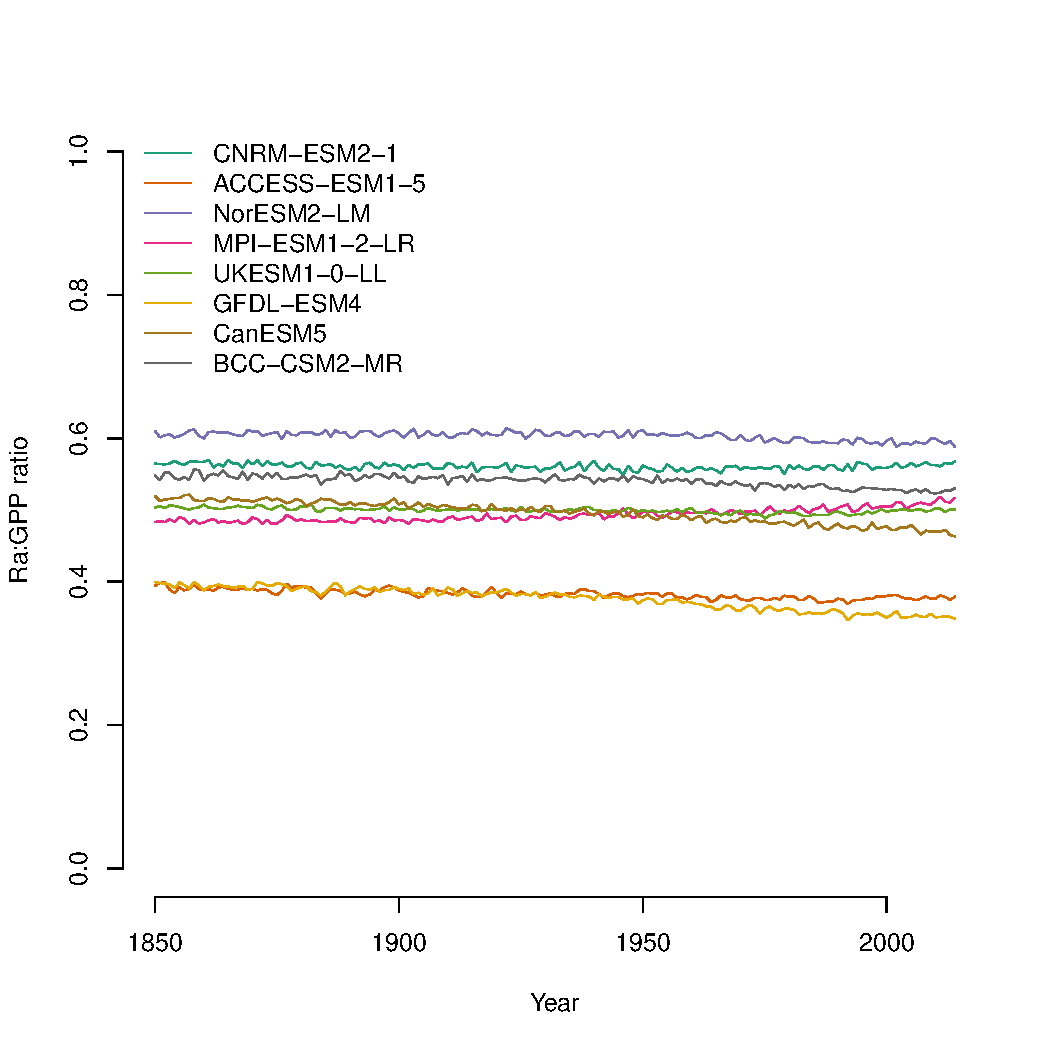
\includegraphics[scale=0.8]{annualRaGPP.pdf} %%%
%DIF <  requires the graphicx package
   %DIFDELCMD < \caption{%
{%DIFAUXCMD
\DIFdelFL{Ratio of autotrophic respiration Ra to gross primary production GPP at the global scale obtained from the historical simulations (}\emph{\DIFdelFL{esm-hist}}%DIFAUXCMD
\DIFdelFL{) of coupled carbon-climate models from the CMIP6 archive. Results from the majority of models suggest that Ra is represented as a constant proportion of GPP that does not change over time despite the increase in GPP predicted by all models.}}
   %DIFAUXCMD
%DIFDELCMD < \label{fig:annualRaGPP}
%DIFDELCMD < \end{figure}
%DIFDELCMD < %%%
\DIFdelend %DIF > \begin{figure}[t]
%DIF >    \centering
%DIF >    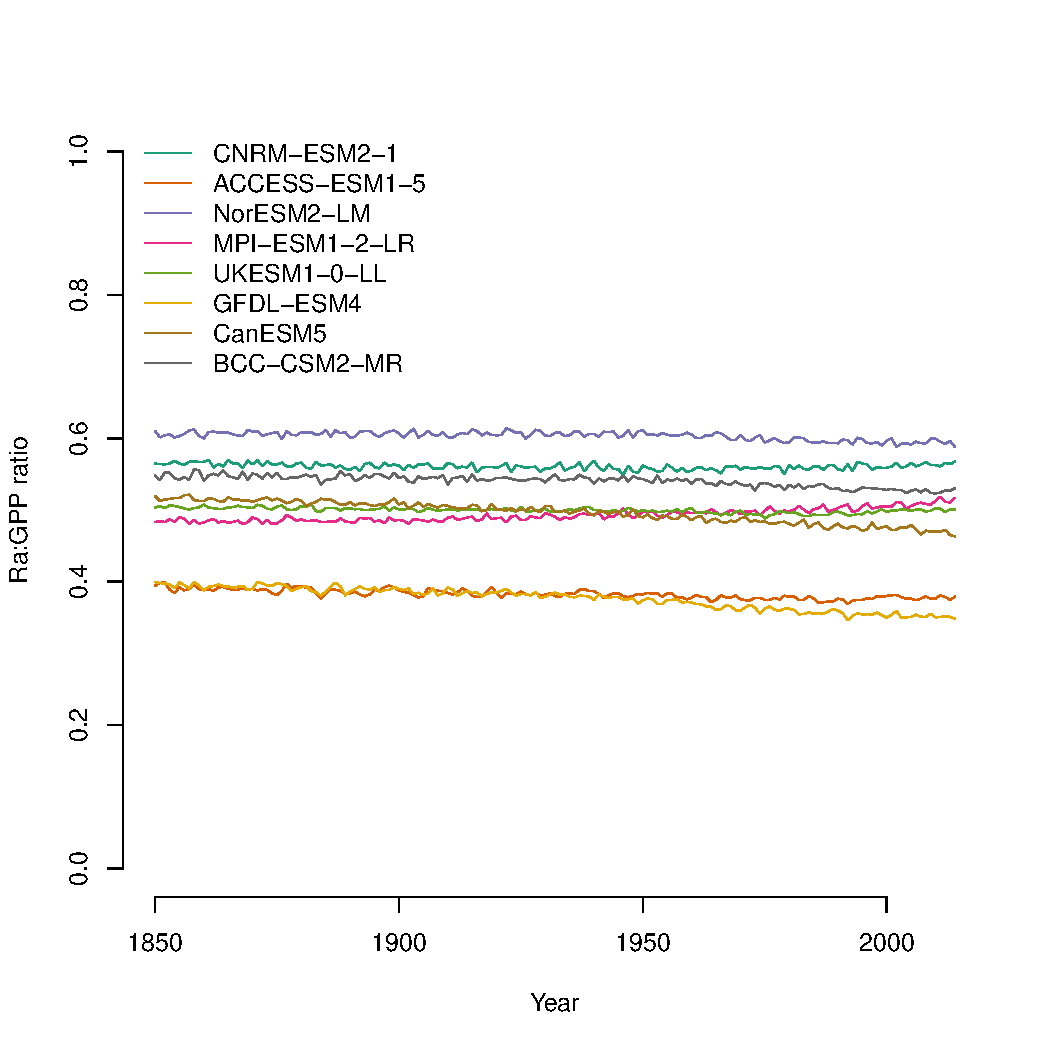
\includegraphics[scale=0.8]{annualRaGPP.pdf} % requires the graphicx package
%DIF >    \caption{Ratio of autotrophic respiration Ra to gross primary production GPP at the global scale obtained from the historical simulations (\emph{esm-hist}) of coupled carbon-climate models from the CMIP6 archive. Results from the majority of models suggest that Ra is represented as a constant proportion of GPP that does not change over time despite the increase in GPP predicted by all models.}
%DIF >    \label{fig:annualRaGPP}
%DIF > \end{figure}

In individual plants, carbon allocation is a highly dynamic process that changes during plant ontogeny to allow them to respond to changes in the environment. \DIFdelbegin \DIFdel{The assumption that Ra is a fixed proportion of GPP does not allow accounting for this dynamic }\DIFdelend \DIFaddbegin \DIFadd{Carbon allocation to individual plant parts and their corresponding respiration is often decoupled from GPP and biomass }\DIFaddend \citep{Collalti2019}. For example, when plants become carbon limited, as it may happen during environmental stress like drought, cold or defoliation, the proportional provision of carbon to Ra decreases, likely to free up resources to maintain allocation to defense \citep{Huang2019EEB,Huang2019NP}. Plant parts that are cut off from canopy photosynthate supply (and thus from GPP) via girdling respire carbon that is years to decades old \citep{muhr:2013}, where Ra is then fueled with carbohydrates that are stored in older tissues. During environmental stress, and during release of stress, belowground Ra recovers faster than assimilation \citep{Hagedorn2016}, again highlighting a situation where Ra is decoupled from GPP \DIFaddbegin \DIFadd{and biomass}\DIFaddend .

A more mechanistic representation of Ra and carbon allocation in models would improve predictions of the dynamic response of terrestrial ecosystems to environmental changes. In particular, the source of the carbon (GPP or NPP) used for carbon allocation in models have consequences to predict the timescale of ecosystem responses as we will show here. 
Consequently, in this manuscript we: (1) review models and conceptual frameworks on the main approaches used to represent Ra and carbon allocation at the ecosystem level; (2) show that models that allocate carbon from NPP and not from GPP predict a transit time equal to zero for the entire autotrophic respiration flux, or in other words, respired carbon from vegetation pools has an age (time since assimilation) equal to zero; (3) demonstrate that this prediction is inconsistent with measurements of the age of respired carbon obtained with radiocarbon measurements and does not capture the variability in the transit time of carbon within vegetation; (4) highlight that the choice of carbon allocation approach has consequences for predicting isotopic exchange fluxes with the atmosphere, to predict the transit time distribution of carbon in the terrestrial biosphere, and to incorporate radiocarbon measurements in model-data assimilation. 

\section{Historical context, concepts, and models}
\subsection{Conceptual support for allocating carbon from NPP}
A common \DIFdelbegin \DIFdel{assumption in ecosystem carbon models is that autotrophic respiration is }\DIFdelend \DIFaddbegin \DIFadd{approach to represent autotrophic respiration (Ra) in ecosystem models is to obtain Ra as }\DIFaddend a constant proportion of GPP\DIFdelbegin \DIFdel{. This assumption }\DIFdelend \DIFaddbegin \DIFadd{, and subsequently allocate NPP to different vegetation pools. This approach }\DIFaddend is based on the work of \citet{Waring1998}, who found constant proportions between NPP and GPP in forest ecosystems, with a constant ratio NPP/GPP = 0.47, or Ra/GPP = 0.53. These constant ratios  promoted  a simplification in the representation of production and growth in models, with NPP \DIFdelbegin \DIFdel{and autotrophic respiration }\DIFdelend often computed as \DIFdelbegin \DIFdel{a proportion (approximately }\DIFdelend 50\% \DIFdelbegin \DIFdel{) }\DIFdelend of annual GPP. Synthesis studies have challenged the constancy of these ratios for different biomes, stand ages, climates, and soils \citep{DeLucia2007, Collalti2019}. 
\DIFdelbegin \DIFdel{Despite criticisms, these simple ratios continue being used as a practical approach to represent Rain many ecosystem models , particularly if the research questions involved only concern net fluxes of carbon between ecosystems and the atmosphere, and not the processes involved in carbon assimilation, allocation to different tissues, and different forms of respiration. 
}\DIFdelend \DIFaddbegin \DIFadd{Although some models may continue using a constant ratio to obtain Ra, many other models have now more dynamic implementations to obtain Ra. Nevertheless, the practice of removing Ra immediately after computing GPP, and subsequently allocating NPP to different plant parts seems to be common to most models. 
%DIF > Despite criticisms, these simple ratios continue being used as a practical approach to represent Ra in many ecosystem models, particularly if the research questions involved only concern net fluxes of carbon between ecosystems and the atmosphere, and not the processes involved in carbon assimilation, allocation to different tissues, and different forms of respiration.
}\DIFaddend 


Although a large proportion ($\sim 50\%$) of assimilated carbon may be respired on an annual basis from ecosystems as postulated by \citet{Waring1998}, this carbon is not necessarily fixed from the current year or growing season. Instead, photo-assimilates and structural tissues of different ages contribute to the total respiratory flux as we will see below.

\citet{Amthor2000} identified three main paradigms generally used to conceptualize the process of autotrophic respiration: (1) the growth-and-maintenance-respiration paradigm (GMRP), (2) the growth-and-maintenance-and-wastage-respiration paradigm (GMWRP), (3) and the general paradigm (GP) that recognizes all possible processes that respiration might support. 

These paradigms are very important to conceptualize the main processes of plant metabolism involved in respiration, but they are not necessarily explicit about the source of carbon that would contribute to the respiration flux. For instance, one can implement a model that computes Ra following the GMWRP, but the actual carbon used for respiration can be subtracted directly from GPP following \citeauthor{Waring1998}'s \citeyearpar{Waring1998} \DIFdelbegin \DIFdel{idea}\DIFdelend \DIFaddbegin \DIFadd{approach}\DIFaddend . Carbon would not enter any plant part, but still it would be respired following some physiological concepts. 

Research on the matrix approach \citep{Luo2017}, which shows that one single equation generalizes the majority of existing ecosystem and land-surface models, suggests that Ra is generally subtracted directly from GPP independently of the respiration paradigm implemented in the model.
The matrix representation of \citet{Luo2017} can be written as

\begin{equation} \label{eq:Luomodel}
\frac{\mathrm{d} \bm{x}}{\mathrm{d}t} =  U(t) \, \bm{b} - \xi(t) \mathbf{A} \, \mathbf{K} \, \bm{x},
\end{equation}
where $\bm{x}$ is a vector of ecosystem carbon pools, $U(t)$ is a function of carbon inputs to the ecosystem, generally obtained as $U(t) = \mathrm{GPP}(t) - \mathrm{Ra}(t) = \mathrm{NPP}(t)$. Then, NPP is allocated to ecosystem compartments such as foliage, wood, and belowground biomass according to the vector of allocation coefficients $\bm{b}$. The product of the matrices $\xi(t)$,  $\mathbf{A}$, and $\mathbf{K}$, is a compartmental matrix that has in its main diagonal the rates at which carbon is processed in each of the compartments, and in its off-diagonal the rates of carbon transfer among compartments. For vegetation compartments, 100\% of all outputs (from mortality and litterfall) are transferred to litter and soil pools, because autotrophic  respiration is already accounted for in the first term of  equation \eqref{eq:Luomodel}. This modeling choice implies that the carbon used for autotrophic respiration never enters a particular vegetation compartment and does not spend any time there (Figure \ref{fig:concept}).

\begin{figure}[t]
   \centering
   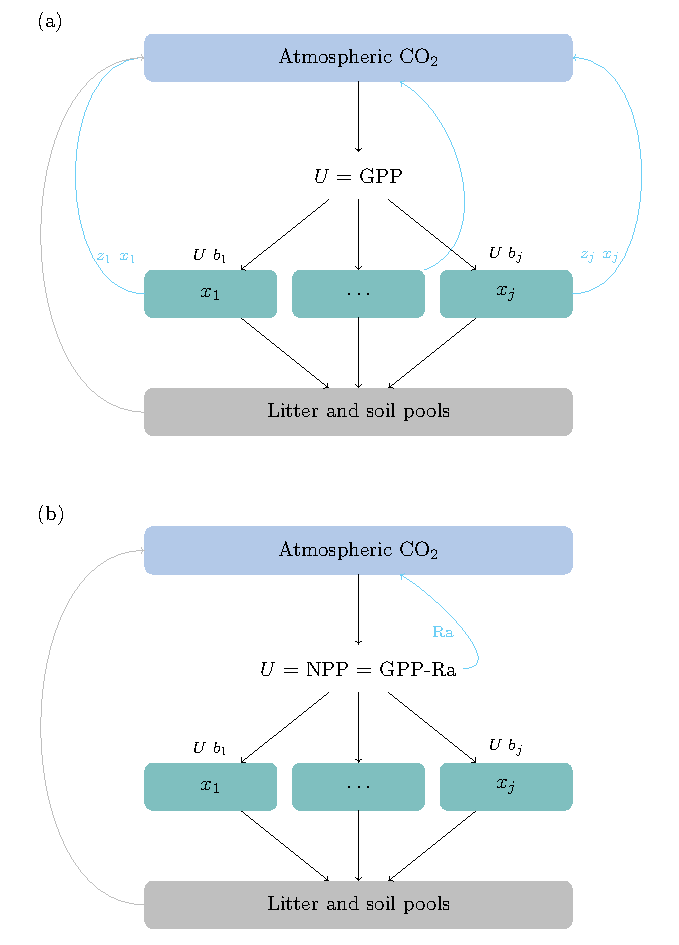
\includegraphics{diagram/conceptualDiagram.pdf} % requires the graphicx package
   \caption{Conceptual diagram representing the difference between allocation schemes. (a) The source of carbon for allocation is GPP, split among the different vegetation pools ($x_1, \dots , x_j$) according to partitioning coefficients ($b_1, \dots , b_j$). The source of carbon for autotrophic respiration is the stock in the vegetation pools and it is computed according to the release coefficients $z_1, \dots , z_j$ (see text for the definition of symbols). (b) The source of carbon allocation is NPP. In this case the functions used to obtain Ra may depend on the stock of carbon or nitrogen in vegetation pools, but Ra is subtracted from GPP before NPP is allocated. The carbon used for Ra never enters the vegetation pools and does not spend any time there.}
   \label{fig:concept}
\end{figure}

In addition to modeling studies, the concept of quantifying carbon allocation after accounting for autotrophic respiration losses is also used in some empirical studies. For instance, the conceptual framework often used to analyze inventory data in tropical forests \citep[e.g.][]{Malhi2011, Malhi2015} assumes that biomass growth results from the allocation of the products of NPP, after autotrophic respiration occurs. In this case however, carbon allocation is understood as \emph{partitioning} of total NPP. \citet{Litton2007} showed that carbon allocation can be understood differently by different authors, as a flux, as biomass, or as partitioning of the total GPP flux. In the case of the tropical forest data, carbon allocation is understood as partitioning coefficients of the NPP flux and not partitioning of GPP as originally defined by \citet{Litton2007}.  

Together, these previous studies show that empirical work has promoted the implementation of Ra as a \DIFdelbegin \DIFdel{constant }\DIFdelend proportion of GPP, or based on some respiration paradigms, but subtracting Ra from GPP before carbon allocation occurs. Therefore models compute first NPP and subsequently allocate the non-respired carbon to plant parts (Figure \ref{fig:concept}). Any model that could be written using the matrix equation with $U = \mathrm{NPP}$ (equation \ref{eq:Luomodel}) would allocate the products of NPP and not GPP, independent of the respiration paradigm described by \citet{Amthor2000}. 

In the following section, we look with more detail at the structure of some particular models with the aim of exploring the main source of carbon used for respiration and allocation.


\subsection{Representation of C allocation in models} 
We reviewed the mathematical structure of \DIFdelbegin \DIFdel{18 }\DIFdelend \DIFaddbegin \DIFadd{19 }\DIFaddend ecosystem models, with particular attention to the functions implemented for \DIFaddbegin \DIFadd{autotrophic }\DIFaddend respiration and carbon allocation. We found that \DIFdelbegin \DIFdel{half of the models (nine) }\DIFdelend \DIFaddbegin \DIFadd{eleven of these models }\DIFaddend calculate a net carbon gain by subtracting both growth and maintenance respiration from GPP \DIFaddbegin \DIFadd{before carbon allocation occurs}\DIFaddend . In this group, maintenance respiration is generally computed based on the stock of carbon or nitrogen in vegetation pools, but it is often the case that the source of the respired carbon is the GPP flux and not the carbon stored.
These models include ISAM \citep{ElMasri2013AgricForMeteorol}, IBIS \citep{Foley1996GBC}, CTEM \citep{Arora2005GCB}, HAVANA \citep{Haverd2016Biogeosciences}, JeDi-DGVM \citep{Pavlick2013Biogeosciences}, and  the model proposed by \citet{Trugman2018EcologyLetters}. 
In \DIFaddbegin \DIFadd{CLM4.5 \mbox{%DIFAUXCMD
\citep{Oleson2013} }\hskip0pt%DIFAUXCMD
for example, maintenance respiration depends on temperature and the stock of nitrogen in each structural carbon pool, but the required amount of carbon needed to maintain existing tissue is subtracted from total GPP. In case the respiratory demand is larger than the available C from GPP, a storage pool provides the necessary amount of carbon for maintenance respiration. Growth respiration is computed as a proportion of the new carbon allocated to growth, and occurs immediately after this allocation occurs, i.e. growth respiration is subtracted from new carbon, despite the presence of NSC pools that only support growth \mbox{%DIFAUXCMD
\citep{Oleson2013}}\hskip0pt%DIFAUXCMD
.
In }\DIFaddend ACONITE \citep{Thomas2014GeosciModelDev}, there is a maintenance respiration compartment that receives C from the labile and bud (a pool that stores C before allocation) C compartments, but not from \DIFdelbegin \DIFdel{the }\DIFdelend leaves, wood and roots. In the model proposed by \citet{Murty2000EcolModel} there are different maintenance respiration terms that are subtracted from GPP before allocation, only respiration from the sapwood pool depends on its C stock, while other respiration terms depend on the N stock. In FOREST-BGC \citep{Running1988EcolModel}, growth respiration and available C are calculated yearly, while maintenance respiration is calculated daily from the C stocks, but both respiration variables are subtracted from GPP. 
\DIFaddbegin \DIFadd{Similarly in CABLE \mbox{%DIFAUXCMD
\citep{Wang2010Biogeosciences, Wang2012}}\hskip0pt%DIFAUXCMD
, both maintenance and growth respiration are subtracted from GPP before allocating C from NPP.
}\DIFaddend 

The other \DIFdelbegin \DIFdel{nine }\DIFdelend \DIFaddbegin \DIFadd{eight }\DIFaddend models do not consider an explicit calculation of stock-dependent maintenance respiration, and also allocate carbon from NPP. Some of these models explicitly \DIFdelbegin \DIFdel{claim }\DIFdelend \DIFaddbegin \DIFadd{express }\DIFaddend that given the linear relationship between C canopy respiration and canopy photosynthesis, the autotrophic respiration is a fixed fraction of the total photosynthetic fixation. Some models that fall into this category are 
\DIFdelbegin \DIFdel{CABLE \mbox{%DIFAUXCMD
\citep{Wang2010Biogeosciences}}\hskip0pt%DIFAUXCMD
, }\DIFdelend G'DAY \citep{Comins1993EA}, DALEC \citep{Williams2005GCB}, CASA \citep{Potter1993GlobalBiogeochemCy}, and TECO \citep{Luo2012TE}. Other models, such as the one proposed by \citet{Hilbert1991AnnBot} calculate the net C gain by subtracting dark respiration from GPP. Three other models do not mention respiration at all, and just partition C from a ``rate of biomass production'': CEVSA2 \citep{Gu2010EcologicalComplexity}, the model proposed by \citet{King1993TreePhysiol}, and the model proposed by \citet{DeAngelis2012TheorEcol} whose net carbon production depends on leaf C. 

In many models, GPP and Ra occur at short timescales (half-hourly, hourly, or daily), computing the net carbon gain as an annual integral. Carbon allocation occurs at annual intervals, when the assimilated carbon that is not respired is assigned to a particular vegetation compartment. Therefore, the carbon that is respired at an intra-annual timescale never enters the vegetation pools.

The important point that we want to highlight here is that even though some models compute maintenance respiration based on knowledge of the carbon stock that needs to be maintained, this respiration is actually subtracted from GPP to obtain the net carbon gain that is subsequently allocated. Only in a few models, maintenance respiration is subtracted from a carbon stock such as a labile pool or other vegetation compartment, but most models can be written in the form of equation \eqref{eq:Luomodel} with $U(t) = \mathrm{NPP}(t)$. 

\subsection{Continuous- versus discrete-time implementations}
In addition to the issue of the source of carbon (GPP or NPP) used for allocation, there is a related problem in computing the age of Ra that emerges in model implementations that are discrete in time. 
Models based on ordinary differential equations such as those expressed as in equation \eqref{eq:Luomodel} treat time as a continuous variable, but many models are implemented in discrete time steps where the carbon stocks of the previous time step are updated based on the functions defined by the model. % (i.e., $\bm{x}(t+\Delta t) = \bm{x}(t) + \Delta t \cdot f(\bm{x}(t))$). 

For example, in the Allometrically Constrained Growth and Carbon Allocation model (ACGCA, \citet{Ogle2009}) maintenance respiration is released from a transient non-structural carbon (NSC) pool.
The carbon there is used for allocation to labile pools, structural tissue in the tree organs, and for respiration.
It is a transient pool because the carbon is used immediately, which allows freshly assimilated carbon to be used  for maintenance respiration.
There are no issues with this implementation in continuous-time \citep{Herrera2020}, but in discrete-time implementations, at a one-year time-step in particular, a large portion of the carbon from the transient pool
never enters the tree.
The net carbon balance is still correct, but the model does not describe accurately the temporal dynamics of the carbon in the transient pool.

To compute maintenance respiration in this model, carbon can be used immediately and hence never enters the tree. Growth respiration on the other hand, happens at the same time step as carbon is allocated to the tree organs but with a one year time lag, one time step after it entered the transient pool from photosynthesis.
Practically, this means that growth respiration happens one year later than maintenance respiration, and that carbon respired by maintenance has an age of zero. 
This age of respired carbon is not realistic when compared with measurements, which can be obtained at finer temporal resolutions and over a broader range. 

\section{Age of respired carbon obtained as the transit time distribution from models}
The age of respired carbon can be obtained from ecosystem models, but the model structure and the form in which the source of carbon for allocation is represented has an impact on the age of carbon respired from ecosystems. Although most models do not represent carbon age explicitly, it can be computed using different computational approaches.

The age of respired carbon from ecosystem is characterized by its transit time distribution \citep{Bolin1973, Thompson1999, Sierra2021JE}. These distributions can be obtained from ecosystem carbon models using impulse response functions \citep{Thompson1999}, a simulation approach that consists of applying a pulse of carbon to a model at equilibrium, where carbon stocks do not change over time, and then observing the respiration flux after the pulse. These distributions can also be obtained using the analytical formulas developed by \citet{Metzler2018MG} for models at equilibrium, or the approach described in \citet{Metzler2018PNAS} for models out of equilibrium.

The transit time distribution represents the proportions of respired carbon that have different ages, and it is usually a continuous function that results from a mixture of exponential functions \citep{Metzler2018MG}. They can be obtained from any ecosystem model expressed in compartmental form as\DIFaddbegin \footnote{\DIFadd{For simplicity of notation, we use here the mathematical representation for linear autonomous systems, but the same arguments can be demonstrated for non-linear non-autonomous systems. However, the notation would be more complex to express and without additional insights.}}
\DIFaddend \begin{equation}
\frac{\mathrm{d}\bm{x}}{\mathrm{d}t} = \bm{u}(t) + \mathbf{B}(t) \, \bm{x}
\end{equation}
where $\bm{u}(t)$ is a vector of carbon inputs to the system. In the framework of \citet{Luo2017}, $\bm{u}(t) = U(t)\, \bm{b}$. The matrix $\mathbf{B}$ is a compartmental matrix with diagonal elements the cycling rates within the pools, and off-diagonal elements the transfer rates of carbon among the different pools. In the framework of \citet{Luo2017}, $\mathbf{B}(t) = \xi(t) \mathbf{A \ K}$. Respiration from each compartment $j$ can be obtained as the product of the amount of mass present in the system and a rate of release $z_j$, 
\begin{equation}
r_j = z_j \ x_j.
\end{equation}
This rate of release $z$ can be obtained from the compartmental matrix $\mathbf{B}$ as the \DIFaddbegin \DIFadd{negative }\DIFaddend sum of the entries of each column. It represents the fraction of carbon that leaves each pool and is not transferred to any other pool.

The transit time distribution of carbon can be defined as the age of the respired carbon from the pools, and can be expressed as \citep{Metzler2018MG}
\begin{equation} \label{eq:transitTime}
f_T(\tau) = \frac{1}{\Vert \bm{r} \Vert} \sum_j r_j f_{aj}(\tau) =  \frac{1}{\Vert \bm{r} \Vert} \sum_j z_j \ x_j f_{aj}(\tau),
\end{equation}
where $f_{aj} (\tau)$ is the age distribution function for pool $j$ as a function of the variable $\tau$ which represents age. The norm symbol \DIFdelbegin \DIFdel{$\Vert \ \Vert$ }\DIFdelend \DIFaddbegin \DIFadd{$\Vert \cdot \Vert$ }\DIFaddend represents the sum of all elements of the vector. \DIFaddbegin \DIFadd{Equation \ref{eq:transitTime} can be interpreted as the relative contribution of pools of different ages to the total respiration flux, in which each pool contains a mix of carbon of different ages characterized by a pool age distribution $f_a$. 
}\DIFaddend 


 If carbon is allocated from GPP, i.e. $\bm{u}(t) = \mathrm{GPP}(t) \ \bm{b}(t) $, autotrophic respiration can only occur directly from the carbon stored in the pools, and $z_j > 0$ for all pools \DIFaddbegin \DIFadd{where carbon is respired }\DIFaddend (Figure \ref{fig:concept}a). Conversely, if carbon is allocated from NPP, i.e. $\bm{u}(t) = (\mathrm{GPP}(t) - \mathrm{Ra}(t)) \ \bm{b}(t)$, no respiration occurs from vegetation pools and $z_j = 0$ for those pools (Figure \ref{fig:concept}b). We can infer then from equation \eqref{eq:transitTime} that for those pools that do not respire carbon ($z_j = r_j = 0$), their contribution to the transit time distribution is equal to zero.

For illustration purposes, we will show here predictions from the global carbon model developed by \citet{Emanuel1981} and used by \citet{Thompson1999} to represent differences between carbon allocation from GPP versus allocation from NPP. We will refer to these two cases as GPP-based versus NPP-based carbon allocation schemes. \DIFaddbegin \DIFadd{We use the model of \mbox{%DIFAUXCMD
\citet{Emanuel1981} }\hskip0pt%DIFAUXCMD
because of its simplicity, which allows us to study differences in model structure without additional complexity.
}\DIFaddend 

At equilibrium, the GPP-based version of the model shows a continuous distribution of carbon that decreases with transit time (Figure \ref{fig:GPPversusNPP}). A large proportion of carbon is respired very quickly after photosynthetic fixation and smaller quantities are respired later on. In contrast, the NPP-based version of the model predicts that all autotrophically respired carbon has an age of zero, and respiration in later years comes only from heterotrophic pools. The median age of the respired carbon (50\% quantile of the transit time distribution) in the GPP-based version of the model is 2.3 yr, i.e. 50 \% of respired carbon is respired in less than 2.3 years. In contrast, in the NPP-based version of the model the median transit time is 0 yr, because the autotrophic respiration flux, which corresponds to 50 \% of GPP, is removed immediately after photosynthetic fixation. 

\begin{figure}[t]
   \centering
   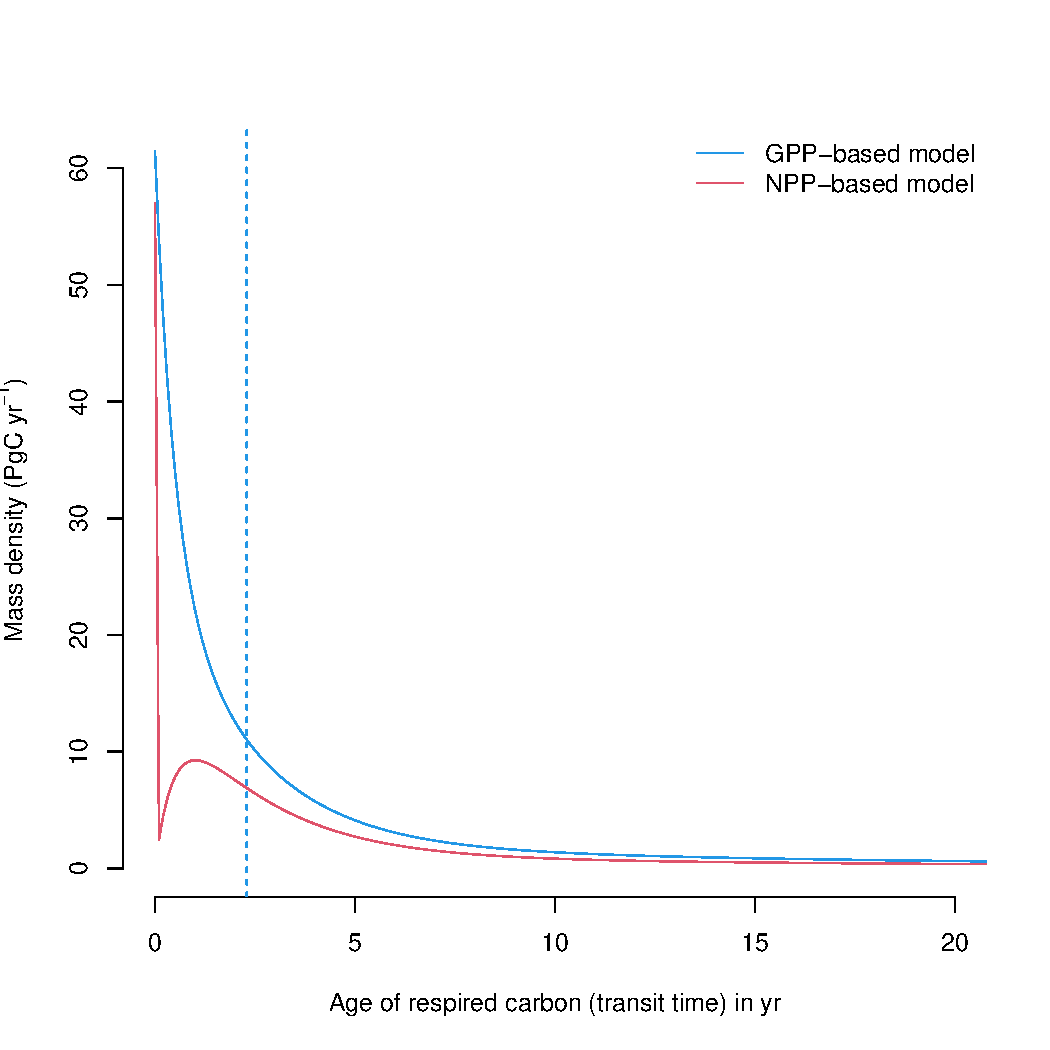
\includegraphics[scale=0.9]{GPPversusNPP_TT.pdf} % requires the graphicx package
   \caption{Transit time distributions obtained from the GPP- and the NPP-based versions of the model of \citet{Emanuel1981}. The vertical dashed line represents the median transit time of the GPP-based model, which is 2.3 yr. For the NPP-version, the median transit time is 0 yr. }
   \label{fig:GPPversusNPP}
\end{figure}

The GPP-based version of the model predicts a continuum of ages of respired carbon both for autotrophic and heterotrophic respiration (Figure \ref{fig:TTcontributions}). Although a large portion of autotrophic respiration is very young ($< 1$ year), a significant proportion is older and can be respired years after photosynthetic fixation. 


\begin{figure}[t]
   \centering
   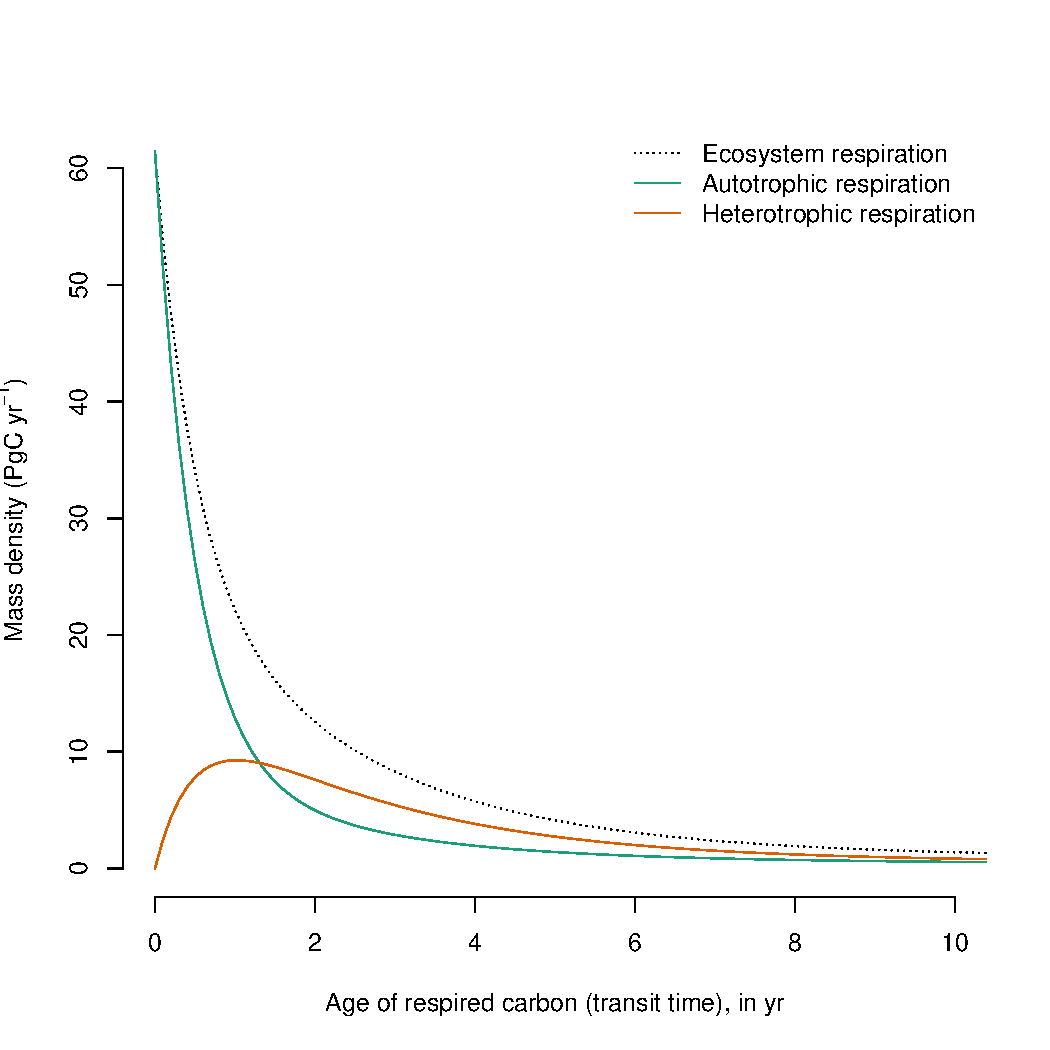
\includegraphics[scale=0.9]{TT_contributions.pdf} % requires the graphicx package
   \caption{Contribution of autotrophic and heterotrophic respiration to the transit time distribution in the GPP-based version of the model of \citet{Emanuel1981}. The age distribution of total ecosystem respiration is equivalent to the transit time distribution of the ecosystem. }
   \label{fig:TTcontributions}
\end{figure}


\section{Age of respired carbon obtained from radiocarbon measurements}
Several studies have used radiocarbon-based methods to estimate the age of the respired carbon form different compartments of the ecosystem (e.g., foliage, wood, roots, and soil) \citep{carbone:2007, Carbone:200713, carbone:2013, muhr:2013, Muhr:2018, Trumbore:2015}. 
In vegetation compartments, studies have focused mostly on individual trees rather than on a larger sample of trees within a forest stand. For healthy mature trees, small differences have been found between compartments, for example carbon respired from leaves may be less than one year old \citep{carbone:2007}, while in roots and stems the respired carbon is on average older than one year, with a mix of carbon from recent assimilates and some contributions of old carbon from storage reserves \citep{Muhr:2018}. There is empirical evidence that shows that the age of the respired carbon by trees can change during different seasons, and increases as trees are exposed to stress and have to use their storage reserves to support metabolic activity.  For instance, \citet{carbone:2013} reported ages of the respired CO$_2$ by the stem of \textit{Acer rubrum} trees of 1.5 and  $\sim$0 yr during spring and late summer, respectively. \citet{muhr:2013} reported ages of 2.5 and 3.3 yr for CO$_2$ respired from the stem of \textit{Simaruba amara} trees during the dry and the wet season, respectively; 2 years old CO$_2$ from the stem of \textit{Tachigali paniculata}; and 4.5 and 4 yr old CO$_2$ from stems of \textit{Hymenolobium pulcherrimum}. Herrera et al (in prep) found similar values as in these previous studies, 5 and 3 years old for CO$_2$ respired by in-stem samples of \textit{Dacriodes microcarpa}, and 2.5 and 5 years old for CO$_2$ from \textit{Ocotea leucoxylon} during the dry  and wet season, respectively. Some studies have also reported several years old respired CO$_2$, ranging from 1 to 5 yr from roots. Most of these studies report mean values of 4 yr old respired carbon from roots \citep{CZIMCZIK:2006td, Schuur:2006tm, carbone:2007}, but younger CO$_2$ (0.6 yr old) has been also reported by \citet{Hilman:2021us}. 

Physical damage such as girdling increases the age of the respired CO$_2$. For example, \citet{Muhr:2018} reported 1 year old CO$_2$ respired by healthy \textit{Scleronema micranthum} trees and 14 years old CO$_2$ respired by trees after one year of girdling. Also, \citet{Hilman:2021us} reported increases in the age of the respired carbon from roots, ranging from \DIFdelbegin \DIFdel{0.6 }\DIFdelend \DIFaddbegin \DIFadd{0.4 }\DIFaddend yr from not girdled trees to \DIFdelbegin \DIFdel{1.3 yr for girdled tress after 1 year}\DIFdelend \DIFaddbegin \DIFadd{1.2 yr for tress after three months of girdling}\DIFaddend .  

With very few exceptions, most of the empirical evidence supports the idea that respired carbon from vegetation parts is on average older than 1 yr, but higher values can be observed depending on the season or on whether trees suffer some form of physiological stress that decreases the supply of recent carbohydrates \citep{Herrera2020}. 

This empirical evidence, which shows that the age of respired carbon spans from one to several years (Figure \ref{fig:ageRespiredC}), is inconsistent with predictions from models in which carbon allocation is based on NPP where the age of respired carbon is exactly equal to zero (Figure \ref{fig:GPPversusNPP}). 

\begin{figure}[t]
   \centering
   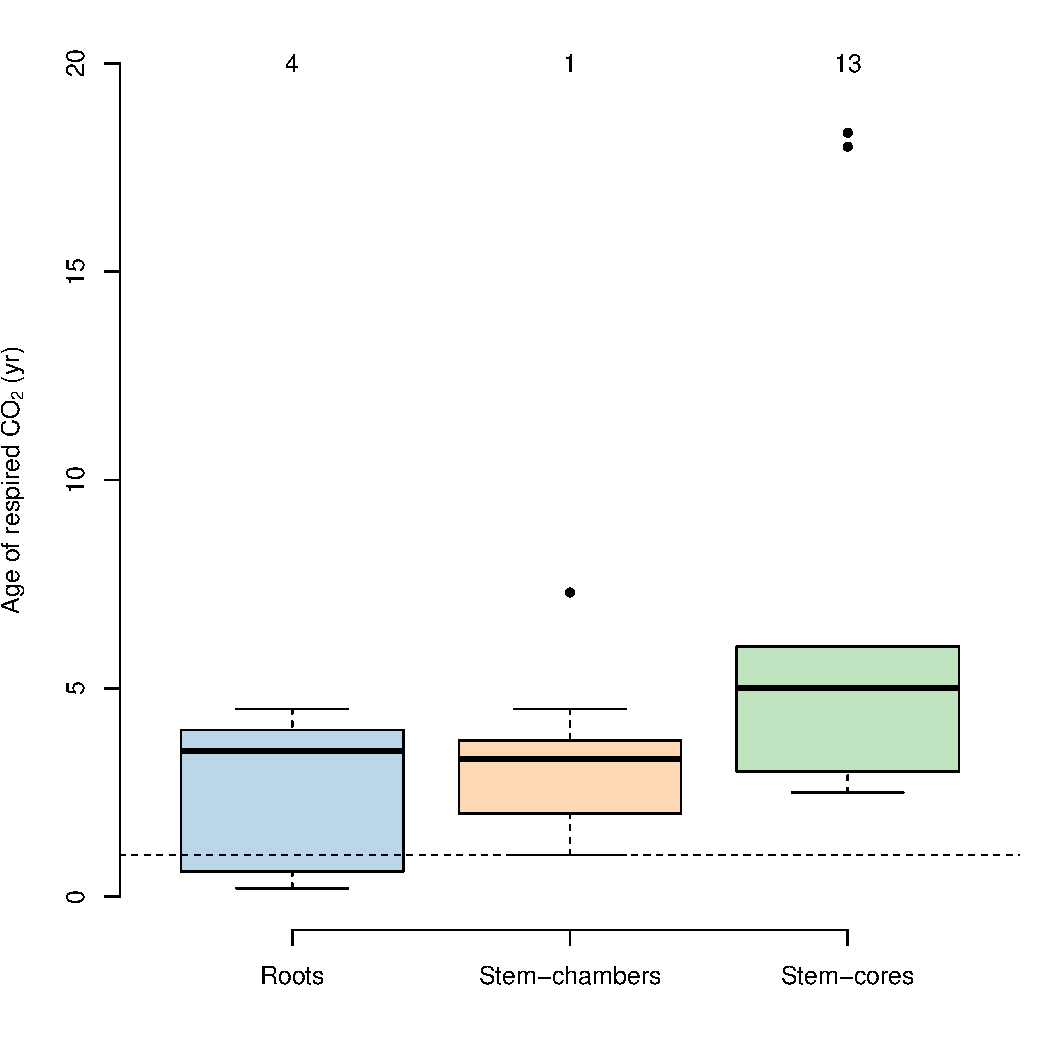
\includegraphics[scale=0.8]{ageRespiredC.pdf} % requires the graphicx package
   \caption{Age of C in respired CO$_2$ from roots and stems for different tree species from temperate and tropical forests obtained from radiocarbon measurements. Data for roots include both fine and coarse roots, and data for stems is split between chamber based measurements and incubations of tree cores. Numbers on top of the boxes represent the number of observations available to draw the boxplots. Values below the horizontal dashed line represent measurements of carbon younger than 1 yr.} 
   \label{fig:ageRespiredC}
\end{figure}


\section{Implications}
The modeling choice of allocating carbon from NPP and not from GPP has important consequences for: (1) use of radiocarbon as an empirical constraint in model-data assimilation studies; (2) computing the transit time distribution of carbon in ecosystems; and (3) determining isotopic exchange between terrestrial ecosystems and the atmosphere. We briefly elaborate on these three implications in the following paragraphs. 

First, as radiocarbon measurements become increasingly available for plant parts and respired CO$_2$ from ecosystems, there is an excellent opportunity to use these data for constraining vegetation models and testing model-based hypotheses. Model-data assimilation techniques are very powerful to reduce model structural uncertainty, and can be used to improve carbon allocation and respiration routines in models.  However, as we have shown here, the age of respired CO$_2$ in NPP-based models is predicted as exactly zero, inconsistent with radiocarbon measurements. Therefore, by construction, NPP-based allocation schemes cannot be used to assimilate radiocarbon measurements and constrain allocation and respiration functions. 

Second, \DIFdelbegin \DIFdel{under the }\DIFdelend \DIFaddbegin \DIFadd{the transit time distribution of carbon is an important metric to integrate many ecosystem-level processes and study ecosystem dynamics \mbox{%DIFAUXCMD
\citep{Bolin1973, Thompson1999, Sierra2017GCB}}\hskip0pt%DIFAUXCMD
. Under the }\DIFaddend assumption of equilibrium, mean transit times of carbon in ecosystems can be obtained by dividing the total carbon stock over the total input flux. However, this approach provides no information on its underlying probability distribution. As shown above, the median transit time can deviate strongly from the mean, and the possibility to compute entire transit time distributions provides very useful information to integrate processes occurring at very different timescales \citep{Sierra2021JE}. Models that subtract autotrophic respiration from GPP before allocating to plant parts cannot be used to compute entire transit time distributions, missing on an opportunity to improve our understanding of the timescales of carbon exchange between ecosystems and the atmosphere. 

Third, the choice of allocation scheme also has consequences for predicting the isotopic exchange of carbon between ecosystems and the atmosphere. For instance, predictions of radiocarbon signatures of respired CO$_2$ from the terrestrial biosphere show a large difference between the GPP- and NPP-based versions of the simple model (Figure \ref{fig:radiocarbon}). Because carbon spends less time in NPP-based allocation schemes, the isotopic exchange between plant parts and the atmosphere occurs more rapidly than in the GPP-based representations.
These differences may have important implications for predicting the isotopic disequilibrium between carbon reservoirs at the Earth system level \DIFdelbegin \DIFdel{\mbox{%DIFAUXCMD
\citep{Randerson2002, Levin2021}}\hskip0pt%DIFAUXCMD
. }\DIFdelend \DIFaddbegin \DIFadd{\mbox{%DIFAUXCMD
\citep{Randerson2002, Levin2021, Frischnecht2022}}\hskip0pt%DIFAUXCMD
. In a recent study, \mbox{%DIFAUXCMD
\citet{Frischnecht2022} }\hskip0pt%DIFAUXCMD
reported that radiocarbon is exchanged too fast in the vegetation component of CLM5.0, inconsistent with previous reconstructions on the incorporation of radiocarbon in the terrestrial biosphere. A potential explanation for the inconsistencies identified by \mbox{%DIFAUXCMD
\citet{Frischnecht2022} }\hskip0pt%DIFAUXCMD
may be the return of radiocarbon in Ra to the atmosphere immediately after GPP due to its allocation scheme. 
}\DIFaddend 

\begin{figure}[t]
   \centering
   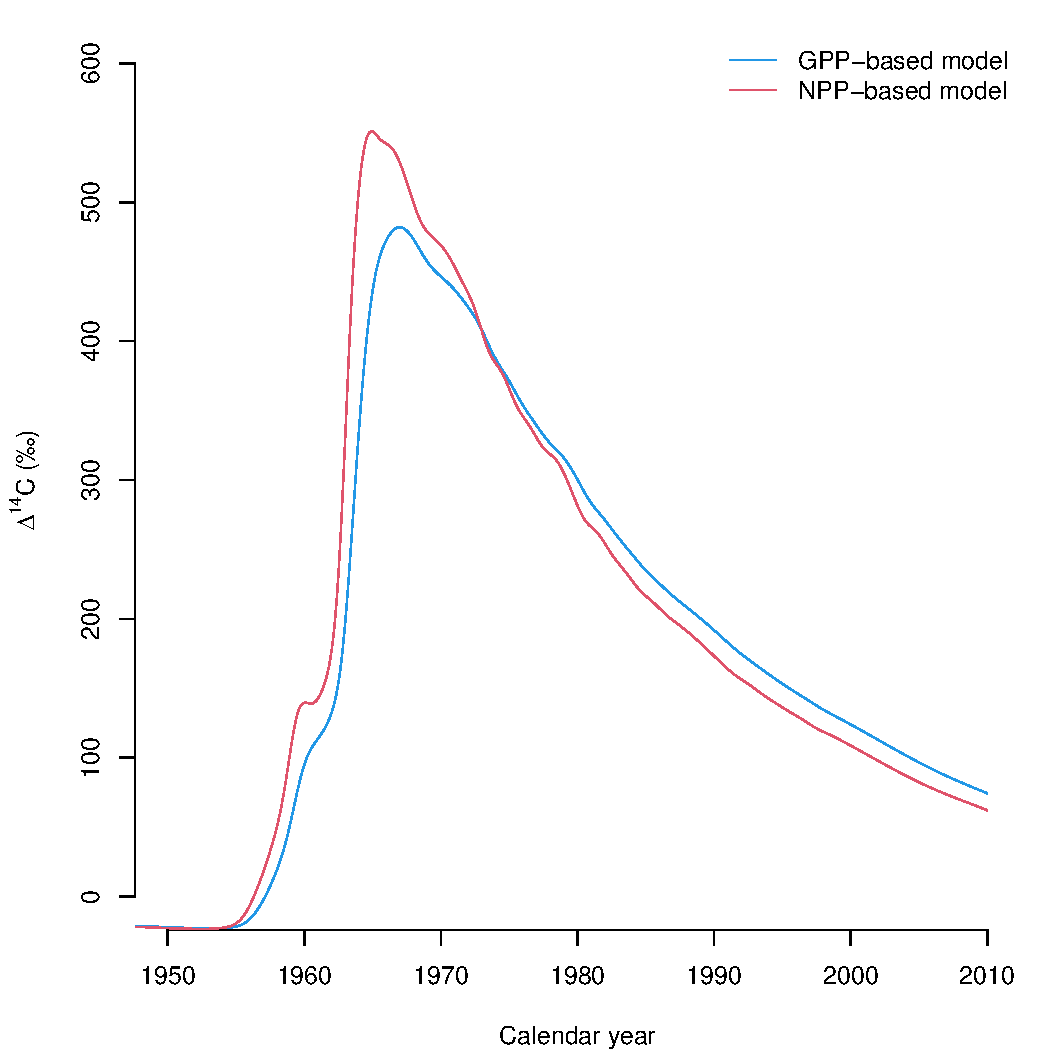
\includegraphics[scale=0.9]{radiocarbon.pdf} % requires the graphicx package
   \caption{Radiocarbon in respired CO$_2$ (in $\Delta^{14}$C) predicted by the two versions of the simple model of \citet{Emanuel1981}. The version in which carbon allocation occurs after Ra is subtracted from GPP (NPP-based model) predicts a faster exchange of radiocarbon with the atmosphere than the GPP-based version of the model where carbon stays for a longer time in the ecosystem.}
   \label{fig:radiocarbon}
\end{figure}


\conclusions[Summary and recommendations]  %% \conclusions[modified heading if necessary]
We have shown that models in which carbon allocation occurs after autotrophic respiration is subtracted from GPP (i.e. NPP-based models) predict that the age of respired carbon from vegetation pools is zero. This prediction contradicts empirical evidence based on the isotopic signature of respired CO$_2$ from plant parts, and suggests that GPP-based allocation schemes are more appropriate to represent carbon allocation and respiration in models. Models in which allocation is based on NPP miss on the opportunity to use radiocarbon data for constraining model parameters and improve their representation of vegetation processes. They are also unable to produce realistic transit time distributions of carbon, and can provide misleading predictions of isotopic exchange between ecosystems and the atmosphere. 

We recommend modeling teams to revise the functions used to compute autotrophic respiration in models, in particular allowing carbon to enter into vegetation pools and then subtracting the autotrophic respiration flux from the standing carbon stock. The addition of a non-structural carbohydrate \DIFaddbegin \DIFadd{(NSC) }\DIFaddend pool can help to improve the dynamics of active carbon that is used to maintain metabolic processes \DIFdelbegin \DIFdel{\mbox{%DIFAUXCMD
\citep{Herrera2020}}\hskip0pt%DIFAUXCMD
}\DIFdelend \DIFaddbegin \DIFadd{\mbox{%DIFAUXCMD
\citep{Ogle2009, Ceballos2018BG, Herrera2020}}\hskip0pt%DIFAUXCMD
}\DIFaddend , but models must ensure that the respired carbon is removed from these NSC pools and not from GPP. \DIFdelbegin \DIFdel{Also, }\DIFdelend \DIFaddbegin \DIFadd{Models with one or two NSC pools can predict age distributions of C that span years to decades \mbox{%DIFAUXCMD
\citep{Trumbore:2015, Ceballos2018BG, Herrera2020}}\hskip0pt%DIFAUXCMD
, consistent with observed data on the radiocarbon of NSCs and of respired CO$_2$. Similar modeling approaches can be implemented in other models. Nevertheless,
}\DIFaddend care must be taken in avoiding artifacts introduced by the time step of the model in discrete-time implementations that may introduce time lags in the use of carbon for respiration. \DIFaddbegin \DIFadd{Differences in the time-step of discrete processes (e.g. GPP computed half-hourly versus annual allocation) pose important challenges for developing GPP-based allocation schemes.  Future research should focus on developing strategies to collect the carbon produced at fast time scales and allocating carbon at monthly or seasonal scales. Data on phenology \mbox{%DIFAUXCMD
\citep{richardson2009, Richardson2018} }\hskip0pt%DIFAUXCMD
and tree-ring formation \mbox{%DIFAUXCMD
\citep{Giraldo2022} }\hskip0pt%DIFAUXCMD
can provide interesting insights for developing new C allocation functions at higher temporal resolution. 
}\DIFaddend 

\DIFaddbegin \DIFadd{Another potential challenge to implement GPP-based carbon allocation schemes may be the availability and quality of GPP data. Traditionally, measurements of NPP and its components have been used to parameterize C allocation schemes, but new allocation functions may need to rely more on GPP data, NSC stocks, and radiocarbon measurements, integrated through data assimilation methods. Eddy-covariance estimates of GPP \mbox{%DIFAUXCMD
\citep{Beer2010}}\hskip0pt%DIFAUXCMD
, together with new data on sun-induced fluoresce \mbox{%DIFAUXCMD
\citep{Gu2019} }\hskip0pt%DIFAUXCMD
are providing now a wealth of data from a large number of ecosystems world wide. Synthesis efforts such as Fluxnet \mbox{%DIFAUXCMD
\citep{Pastorello2020} }\hskip0pt%DIFAUXCMD
and Fluxcom \mbox{%DIFAUXCMD
\citep{Jung2020} }\hskip0pt%DIFAUXCMD
provide well-curated data-products of global GPP. In particular, Fluxcom combines remote sensing information with eddy-flux data to produce global gridded products of GPP at high spatial and temporal resolution, which could be of immense value for modeling studies. 
}

\DIFaddend Radiocarbon measurements in respired CO$_2$ from plant parts and whole ecosystem pools can \DIFaddbegin \DIFadd{also }\DIFaddend greatly help to test the mathematical structure of autotrophic respiration and allocation functions in models. These measurements are only available for a small set of sites, but future efforts should expand to more diverse ecosystems, capturing patterns induced by environmental drivers.  Assimilation of radiocarbon data into ecosystem models offers large opportunities to improve our overall understanding of the timescales of carbon cycling in ecosystems and how they respond to environmental change. 

%% The following commands are for the statements about the availability of data sets and/or software code corresponding to the manuscript.
%% It is strongly recommended to make use of these sections in case data sets and/or software code have been part of your research the article is based on.

%\codeavailability{} %% use this section when having only software code available


%\dataavailability{TEXT} %% use this section when having only data sets available


\DIFdelbegin %DIFDELCMD < \codedataavailability{All data and code used for this manuscript is available at \url{https://github.com/crlsierra/allocationGPPorNPP}.
%DIFDELCMD < Upon acceptance, a static copy of the repository will be archived in Zenodo and will be cited with a doi.} %%%
%DIF < % use this section when having data sets and software code available
\DIFdelend \DIFaddbegin \codedataavailability{All data and code used for this manuscript is available at \url{https://github.com/crlsierra/allocationGPPorNPP}.}
%DIF > Upon acceptance, a static copy of the repository will be archived in Zenodo and will be cited with a doi.} %% use this section when having data sets and software code available
\DIFaddend 


%\sampleavailability{TEXT} %% use this section when having geoscientific samples available


%\videosupplement{TEXT} %% use this section when having video supplements available


%\appendix
%\section{}    %% Appendix A
%
%\subsection{}     %% Appendix A1, A2, etc.
%
%
%\noappendix       %% use this to mark the end of the appendix section. Otherwise the figures might be numbered incorrectly (e.g. 10 instead of 1).

%% Regarding figures and tables in appendices, the following two options are possible depending on your general handling of figures and tables in the manuscript environment:

%% Option 1: If you sorted all figures and tables into the sections of the text, please also sort the appendix figures and appendix tables into the respective appendix sections.
%% They will be correctly named automatically.

%% Option 2: If you put all figures after the reference list, please insert appendix tables and figures after the normal tables and figures.
%% To rename them correctly to A1, A2, etc., please add the following commands in front of them:

\appendixfigures  %% needs to be added in front of appendix figures

\appendixtables   %% needs to be added in front of appendix tables

%% Please add \clearpage between each table and/or figure. Further guidelines on figures and tables can be found below.



\authorcontribution{CAS designed research and wrote the manuscript. DHR compiled empirical studies on radiocarbon. VCN reviewed literature on models. HM analyzed differences between discrete and continuous implementations of Ra in models. HH wrote sections on physiology. All authors discussed ideas and contributed to writing.} %% this section is mandatory

\competinginterests{The authors declare no competing interests.} %% this section is mandatory even if you declare that no competing interests are present

%\disclaimer{TEXT} %% optional section

\begin{acknowledgements}
Funding was provided by the German Research Foundation (SI 1953/2-2), the Max Planck Society, and the Swedish University for Agricultural Sciences. HM acknowledges the support of the Swedish Research Council for Sustainable Development FORMAS, under grant 2018-01820.
\end{acknowledgements}




%% REFERENCES

%% The reference list is compiled as follows:

%\begin{thebibliography}{}
%
%\bibitem[AUTHOR(YEAR)]{LABEL1}
%REFERENCE 1
%
%\bibitem[AUTHOR(YEAR)]{LABEL2}
%REFERENCE 2
%
%\end{thebibliography}

%% Since the Copernicus LaTeX package includes the BibTeX style file copernicus.bst,
%% authors experienced with BibTeX only have to include the following two lines:
%%
 \bibliographystyle{copernicus}
 \bibliography{../allocationNPP.bib}
%%
%% URLs and DOIs can be entered in your BibTeX file as:
%%
%% URL = {http://www.xyz.org/~jones/idx_g.htm}
%% DOI = {10.5194/xyz}


%% LITERATURE CITATIONS
%%
%% command                        & example result
%% \citet{jones90}|               & Jones et al. (1990)
%% \citep{jones90}|               & (Jones et al., 1990)
%% \citep{jones90,jones93}|       & (Jones et al., 1990, 1993)
%% \citep[p.~32]{jones90}|        & (Jones et al., 1990, p.~32)
%% \citep[e.g.,][]{jones90}|      & (e.g., Jones et al., 1990)
%% \citep[e.g.,][p.~32]{jones90}| & (e.g., Jones et al., 1990, p.~32)
%% \citeauthor{jones90}|          & Jones et al.
%% \citeyear{jones90}|            & 1990



%% FIGURES

%% When figures and tables are placed at the end of the MS (article in one-column style), please add \clearpage
%% between bibliography and first table and/or figure as well as between each table and/or figure.

% The figure files should be labelled correctly with Arabic numerals (e.g. fig01.jpg, fig02.png).


%% ONE-COLUMN FIGURES

%%f
%\begin{figure}[t]
%\includegraphics[width=8.3cm]{FILE NAME}
%\caption{TEXT}
%\end{figure}
%
%%% TWO-COLUMN FIGURES
%
%%f
%\begin{figure*}[t]
%\includegraphics[width=12cm]{FILE NAME}
%\caption{TEXT}
%\end{figure*}
%
%
%%% TABLES
%%%
%%% The different columns must be seperated with a & command and should
%%% end with \\ to identify the column brake.
%
%%% ONE-COLUMN TABLE
%
%%t
%\begin{table}[t]
%\caption{TEXT}
%\begin{tabular}{column = lcr}
%\tophline
%
%\middlehline
%
%\bottomhline
%\end{tabular}
%\belowtable{} % Table Footnotes
%\end{table}
%
%%% TWO-COLUMN TABLE
%
%%t
%\begin{table*}[t]
%\caption{TEXT}
%\begin{tabular}{column = lcr}
%\tophline
%
%\middlehline
%
%\bottomhline
%\end{tabular}
%\belowtable{} % Table Footnotes
%\end{table*}
%
%%% LANDSCAPE TABLE
%
%%t
%\begin{sidewaystable*}[t]
%\caption{TEXT}
%\begin{tabular}{column = lcr}
%\tophline
%
%\middlehline
%
%\bottomhline
%\end{tabular}
%\belowtable{} % Table Footnotes
%\end{sidewaystable*}
%
%
%%% MATHEMATICAL EXPRESSIONS
%
%%% All papers typeset by Copernicus Publications follow the math typesetting regulations
%%% given by the IUPAC Green Book (IUPAC: Quantities, Units and Symbols in Physical Chemistry,
%%% 2nd Edn., Blackwell Science, available at: http://old.iupac.org/publications/books/gbook/green_book_2ed.pdf, 1993).
%%%
%%% Physical quantities/variables are typeset in italic font (t for time, T for Temperature)
%%% Indices which are not defined are typeset in italic font (x, y, z, a, b, c)
%%% Items/objects which are defined are typeset in roman font (Car A, Car B)
%%% Descriptions/specifications which are defined by itself are typeset in roman font (abs, rel, ref, tot, net, ice)
%%% Abbreviations from 2 letters are typeset in roman font (RH, LAI)
%%% Vectors are identified in bold italic font using \vec{x}
%%% Matrices are identified in bold roman font
%%% Multiplication signs are typeset using the LaTeX commands \times (for vector products, grids, and exponential notations) or \cdot
%%% The character * should not be applied as mutliplication sign
%
%
%%% EQUATIONS
%
%%% Single-row equation
%
%\begin{equation}
%
%\end{equation}
%
%%% Multiline equation
%
%\begin{align}
%& 3 + 5 = 8\\
%& 3 + 5 = 8\\
%& 3 + 5 = 8
%\end{align}
%
%
%%% MATRICES
%
%\begin{matrix}
%x & y & z\\
%x & y & z\\
%x & y & z\\
%\end{matrix}
%
%
%%% ALGORITHM
%
%\begin{algorithm}
%\caption{...}
%\label{a1}
%\begin{algorithmic}
%...
%\end{algorithmic}
%\end{algorithm}
%
%
%%% CHEMICAL FORMULAS AND REACTIONS
%
%%% For formulas embedded in the text, please use \chem{}
%
%%% The reaction environment creates labels including the letter R, i.e. (R1), (R2), etc.
%
%\begin{reaction}
%%% \rightarrow should be used for normal (one-way) chemical reactions
%%% \rightleftharpoons should be used for equilibria
%%% \leftrightarrow should be used for resonance structures
%\end{reaction}
%
%
%%% PHYSICAL UNITS
%%%
%%% Please use \unit{} and apply the exponential notation


\end{document}
